\newcommand\tab[1][1cm]{\hspace*{#1}}
\newcommand{\el}{e\textsuperscript{-}}
\chapter[Biochémia]{Biochémia}
\label{biochemia} % id kapitoly pre prikaz ref

%1
\section{Chémia ako logický základ biologického fenoménu DONE}
Status: DONE
Source: Prezentácia 1
\\
\subsection{Základné vlastnosti živých systémov}
Zložité a organizované\\
Bio štruktúry majú funkčný význam\\
Aktívne zapojené do premien energie\\
Schopnosť replikácie\\
Chemický základ
\subsection{Biomolekuly}
HOCN -- schopnosť vytvárať kovalentné väzby cez \el páry $\rightarrow$ rôzne štruktúry
\subsection{Vlastnosti biomolekúl}
Štruktúrna polarita (napr. 5' $\rightarrow$ 3')\\
Informatívnosť (napr. DNA, polypeptidy)\\
Trojrozmerná štruktúra\\
\subsection{Vlastnosti vody}
Vysoká hodnota teploty topenia a varu, výparného tepla, povrchového napätia\\
Polarita $\leftarrow$ Lomená štruktúra\\
Tvorba vodíkových väzieb\\
Solvatačné vlastnosti\\
\tab Polárne látky $\rightarrow$ vodíkové väzby\\
\tab Nepolárne $\rightarrow$ hydrofóbne interakcie
\subsection{Typy a význam slabých interakcií v biologických štruktúrach}
Slabé interakcie udržujú 3D štruktúru a určujú interakcie\\
\tab Napr. biomolekulárne rozpoznávanie\\
\tab Obmedzené vhodné enviromentálne podmienky\\
Van der Waalsove\\
Vodíkové\\
Iónové\\
Hydrofóbne
\subsection{Hydrofóbne interakcie}
Disperzia lipidov $\rightarrow$ usporiadavajú okolitú H2O\\
Lipidy sa zoskupujú $\rightarrow$ entropia systému rastie, výhodnejší stav\\
Micely $\rightarrow$ hydrofóbne konce idú dnu, entropia systému vyššia\\

%2
\section{Aminokyseliny a proteíny DONE}

Status: DONE
Source: Prezentácia 1
\\
\subsection{Všeobecný vzorec AK}
\includegraphics[width=0.25\textwidth, page=35]{materials/Biochemia/Prezentacie_Biochemia/01_Uvod_AK_Proteiny.pdf}
\subsection{Klasifikácia AK}
D, L izoméria\\
rozdelenie na základe chem vlastností side chain\\
\tab náboj\\
\tab schopnosť viazať H\\
\tab Kyslá/zásaditá\\
Nepolárne -- hydrofóbne\\
Polárne -- hydrofilné
\subsection{vzorce AK}
\includegraphics[width=0.5\textwidth, page=37]{materials/Biochemia/Prezentacie_Biochemia/01_Uvod_AK_Proteiny.pdf}
\includegraphics[width=0.5\textwidth, page=38]{materials/Biochemia/Prezentacie_Biochemia/01_Uvod_AK_Proteiny.pdf}
\\
Tvorba disulfidovej väzby

\includegraphics[width=0.5\textwidth, page=39]{materials/Biochemia/Prezentacie_Biochemia/01_Uvod_AK_Proteiny.pdf}
\\
\subsection{optická aktivita}
Schopnosť otáčať rovinu polarizovaného svetla -- napr. Vlnenie fotónu ide zhora dole $\rightarrow$ zľava doprava\\
Všetky AK okrem glycínu\\
L a D aminokyseliny \\

\includegraphics[width=0.5\textwidth, page=44]{materials/Biochemia/Prezentacie_Biochemia/01_Uvod_AK_Proteiny.pdf}
\\
\subsection{spektroskopické vlastnosti AK}
Absorbujú v infrač. oblasti\\
Trp a tyr, menej Phe v UV\\
Absorbcia pri 280nm sa používa pri detekcii proteínov\\
\\
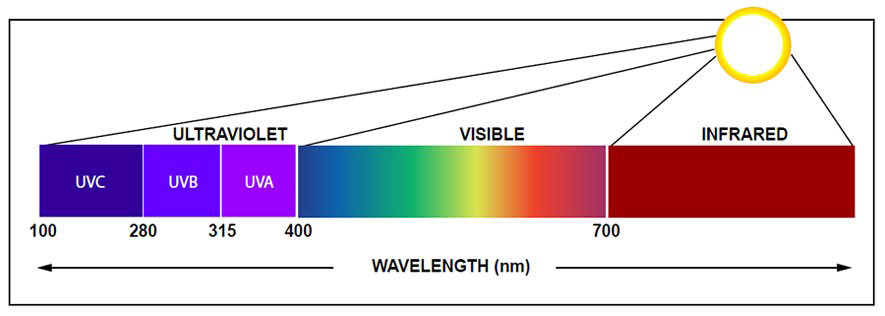
\includegraphics[width=0.5\textwidth]{images/wavelength}
\\
\subsection{acidobázické vlastnosti AK}
Pri nízkom pH je veľa H+, AK stráca čiastočne negatívny náboj a ostane s kladným. \\
Pri vysokom pH je veľa OH-- $\rightarrow$ bude mať záporný náboj\\
\subsection{Zwitterióny, amfotérny charakter AK, }
Pri neutrálnom pH má oba náboje $\rightarrow$ Zwitterión/Amfión\\
Vie reagovať s kys. aj zásadami\\
\subsection{izoelektrický bod}
izoelektrický bod: pH, keď sa AK mení z -- na 0 alebo z + na 0.\\
\tab pI = (pKA kyslého + pKA zásaditého)/2. Obyčajne 9 a 2\\
\tab pI = average of pKAs of functional groups
\subsection{štruktúra a vlastnosti peptidovej väzby}

\includegraphics[width=0.5\textwidth, page=46]{materials/Biochemia/Prezentacie_Biochemia/01_Uvod_AK_Proteiny.pdf}
\\
Odchádza/prichádza H2O\\
N\textsuperscript{+}, O\textsuperscript{-}
medzi jednoduchou a dvojitou\\
trans\\
6 atómov v rovine -- planárne usporiadanie
\subsection{Trojrozmerná štruktúra proteínov}
primárna, sekundárna ($\alpha$--helix, $\beta$--skladaný list, $\beta$--otáčka), terciárna, kvartérna, 
väzby (interakcie) a funkčné skupiny uplatňujúce sa pri jednotlivých štruktúrach\\
\\
Primárna\\
\tab poradie AK, kovalentné peptidové väzby\\
Sekundárna\\
\tab ako sa skladajú na seba, (základná štruktúra, nie zvyšky), vodíkové väzby medzi CO a NH\\
\tab $\alpha$--helix (pravotočivý)\\
\tab \tab Väzba o 4 zvyšky dopredu\\
\tab $\beta$--skladaný list\\
\tab \tab paralelný, antiparalelný\\
\tab \tab Úplne rozvinutý reťazec\\
\tab \tab Väzby aj medzi rozdielnymi reťazcami\\
\tab $\beta$--otáčka\\
\tab \tab Zmena smeru peptidového reťazcu\\
\tab \tab Väzba o 3 zvyšky ďalej\\
\tab \tab prolín, glycín\\
Terciárna\\
\tab Priestorová štruktúra, interakcie vzdialených skupín, ako sa folds skladajú na seba, vodíkové väzby, Van der Waals, hydrofóbny obal, disulfidový mostík medzi bočnými reťazcami\\
\tab Daná primárnou štruktúrou\\
kvartérna\\
\tab medzi rôznymi polypeptidmi\\
\tab podjednotky sa skladajú do mérov -- diméry, tetraméry, multiméry $\rightarrow$ počty polypeptidových reťazcov\\
\tab Homo/hetero multimérne -- rovnaké/rôzne reťazce\\
%TODO: Kedy sa rozpadajú? Zmena pH, teplota, atď?\\
Cysteín -- disulfidový mostík\\

\subsection{Rozdelenie proteínov podľa štruktúry a rozpustnosti (fibrilárne, globulárne, membránové proteíny)}
Fibrilárne\\
\tab pevné, reťazce väčšinou paralelné s jednou osou\\
\tab nerozpustné, štruktúrna funkcia\\
\tab keratíny, kolagén, fibroín\\

\includegraphics[width=0.5\textwidth, page=73]{materials/Biochemia/Prezentacie_Biochemia/01_Uvod_AK_Proteiny.pdf}
\\
Globulárne\\
\tab hydrofilné von, hydrofóbne dnu\\
\tab Flexibilné časti, štruktúry nie sú statické (PARTAAY)\\
\tab mioglobín, cytochróm c, lyzozým, ribonukleáza\\
Membránové\\
\tab bakteriorodospín\\
\subsection{Biologická funkcia proteínov, natívna konformácia, denaturácia, renaturácia}
Enzýmová katalýza\\
Transportná, zásobná -- hemoglobín(O2), sérumalbumín (MK), Ovalbumín, Kazeín (N), Ferritín (Fe)\\
Koordinovaný pohyb -- Aktín, myozín\\
mechanická podpora -- kolagén, keratín\\
Imunita\\
nervové impulzy\\
regulácia rastu, diferenciácia\\
\\
natívna konformácia -- správne zložený proteín. Aktívna forma. Chyby na hociktorej úrovni vedú ku chorobám\\
Denaturácia\\
\tab unfolded, neaktívny\\
\tab pH, teplota, chemikálie, org. rozpúšťadlá, detergenty, močovina, enzýmy\\
\tab Neovplyvňuje primárnu štruktúru.\\
\tab vratná/nevratná\\
Renaturácia\\
\tab Nie vždy sa poskladá správne\\
Chaperone -- proteín, čo skladá správne proteíny\\
Prirodzene neusporiadané proteíny $\rightarrow$ viac funkcií, nemávajú hydrofóbne jadro

%3
\section{Sacharidy}
Status: In progress
Source: Prezentácia 2
\\
\subsection{Rozdelenie sacharidov, aldózy, ketózy}
aldózy -- O na začiatku\\
ketózy -- O v strede\\
mono, oligo, poly\\
lineárne, rozvetvené\\

\subsection{Vzorce}
lineárne -- Fischerove\\
\tab cyklické -- Haworthove: \\

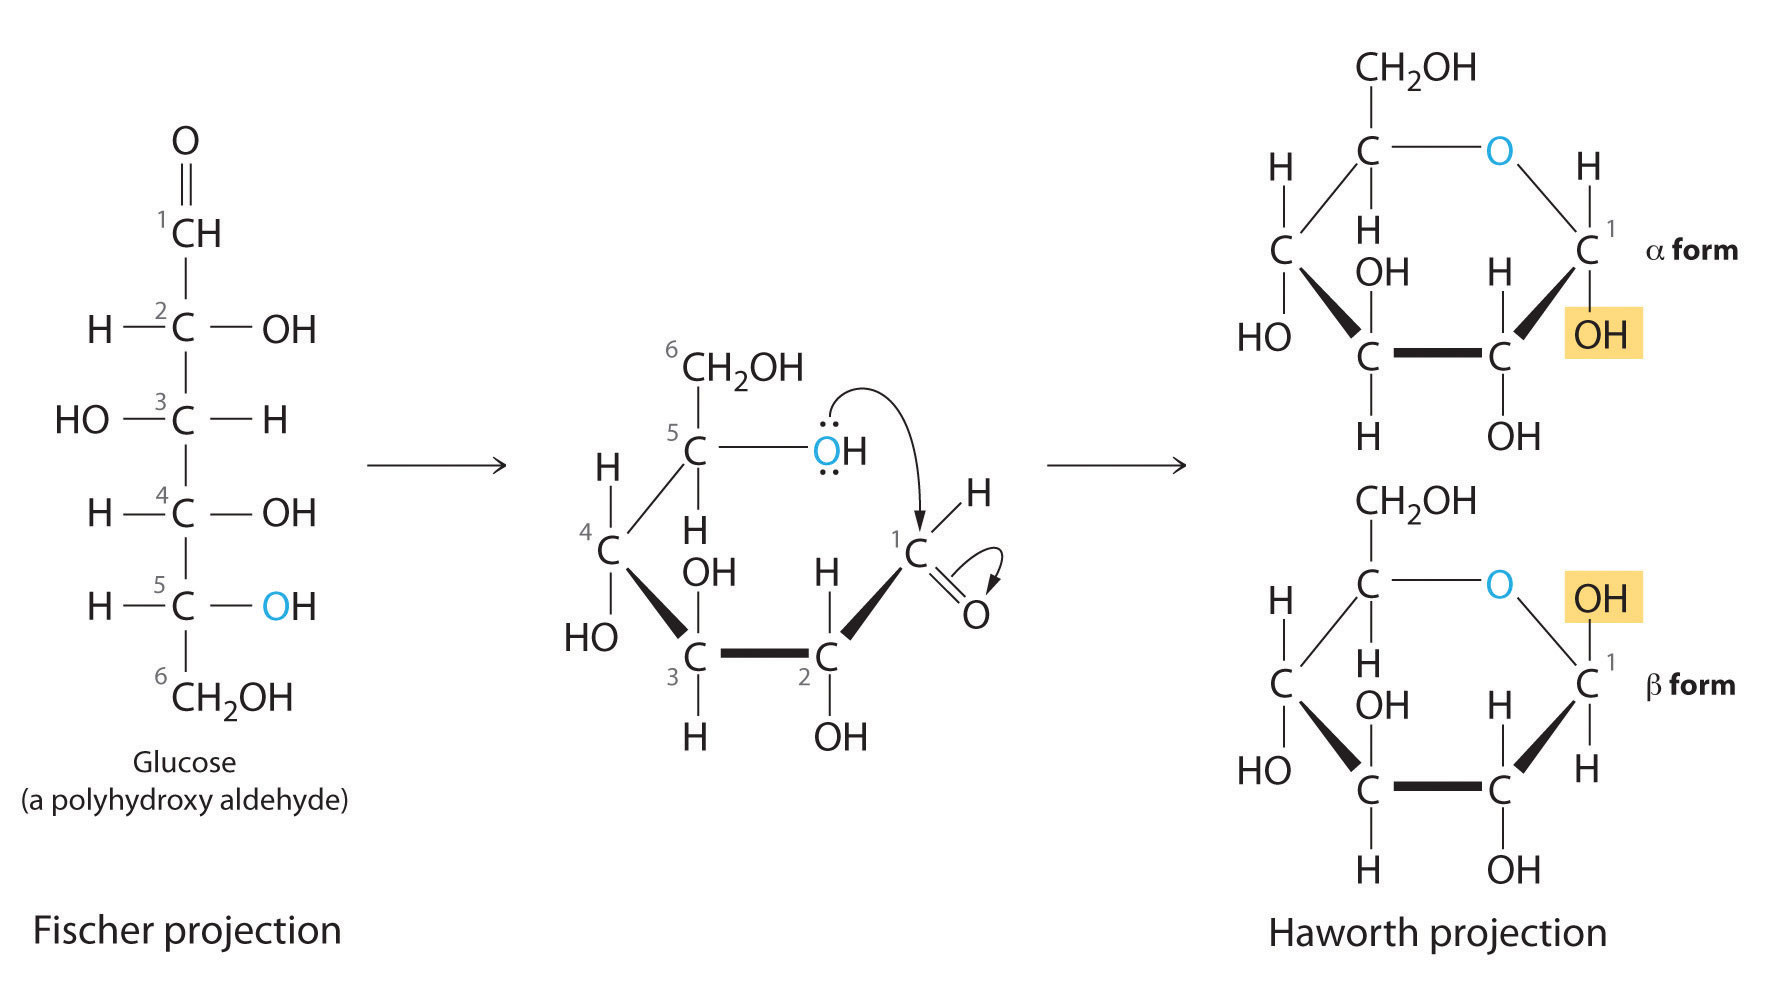
\includegraphics[width=0.5\textwidth]{images/fischer_to_haworth_sacharidy}
\\
D alebo L podľa OH na spodnom chirálnom uhlíku (to je ten druhý uhlík z dola)\\
L je zrkadlové ku D\\
\tab D-glukóza:\\
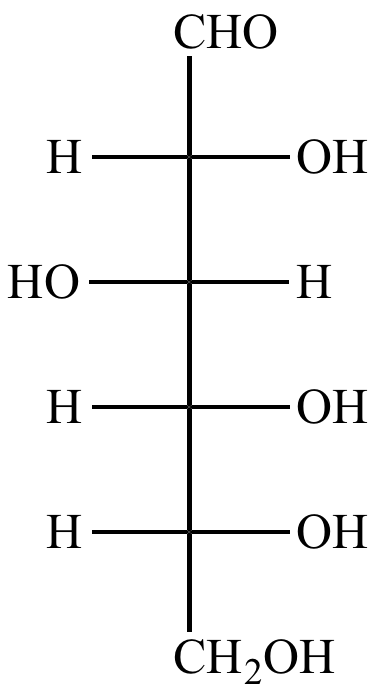
\includegraphics[width=0.2\textwidth]{images/glucose}\\
\\
\tab D-manóza:\\
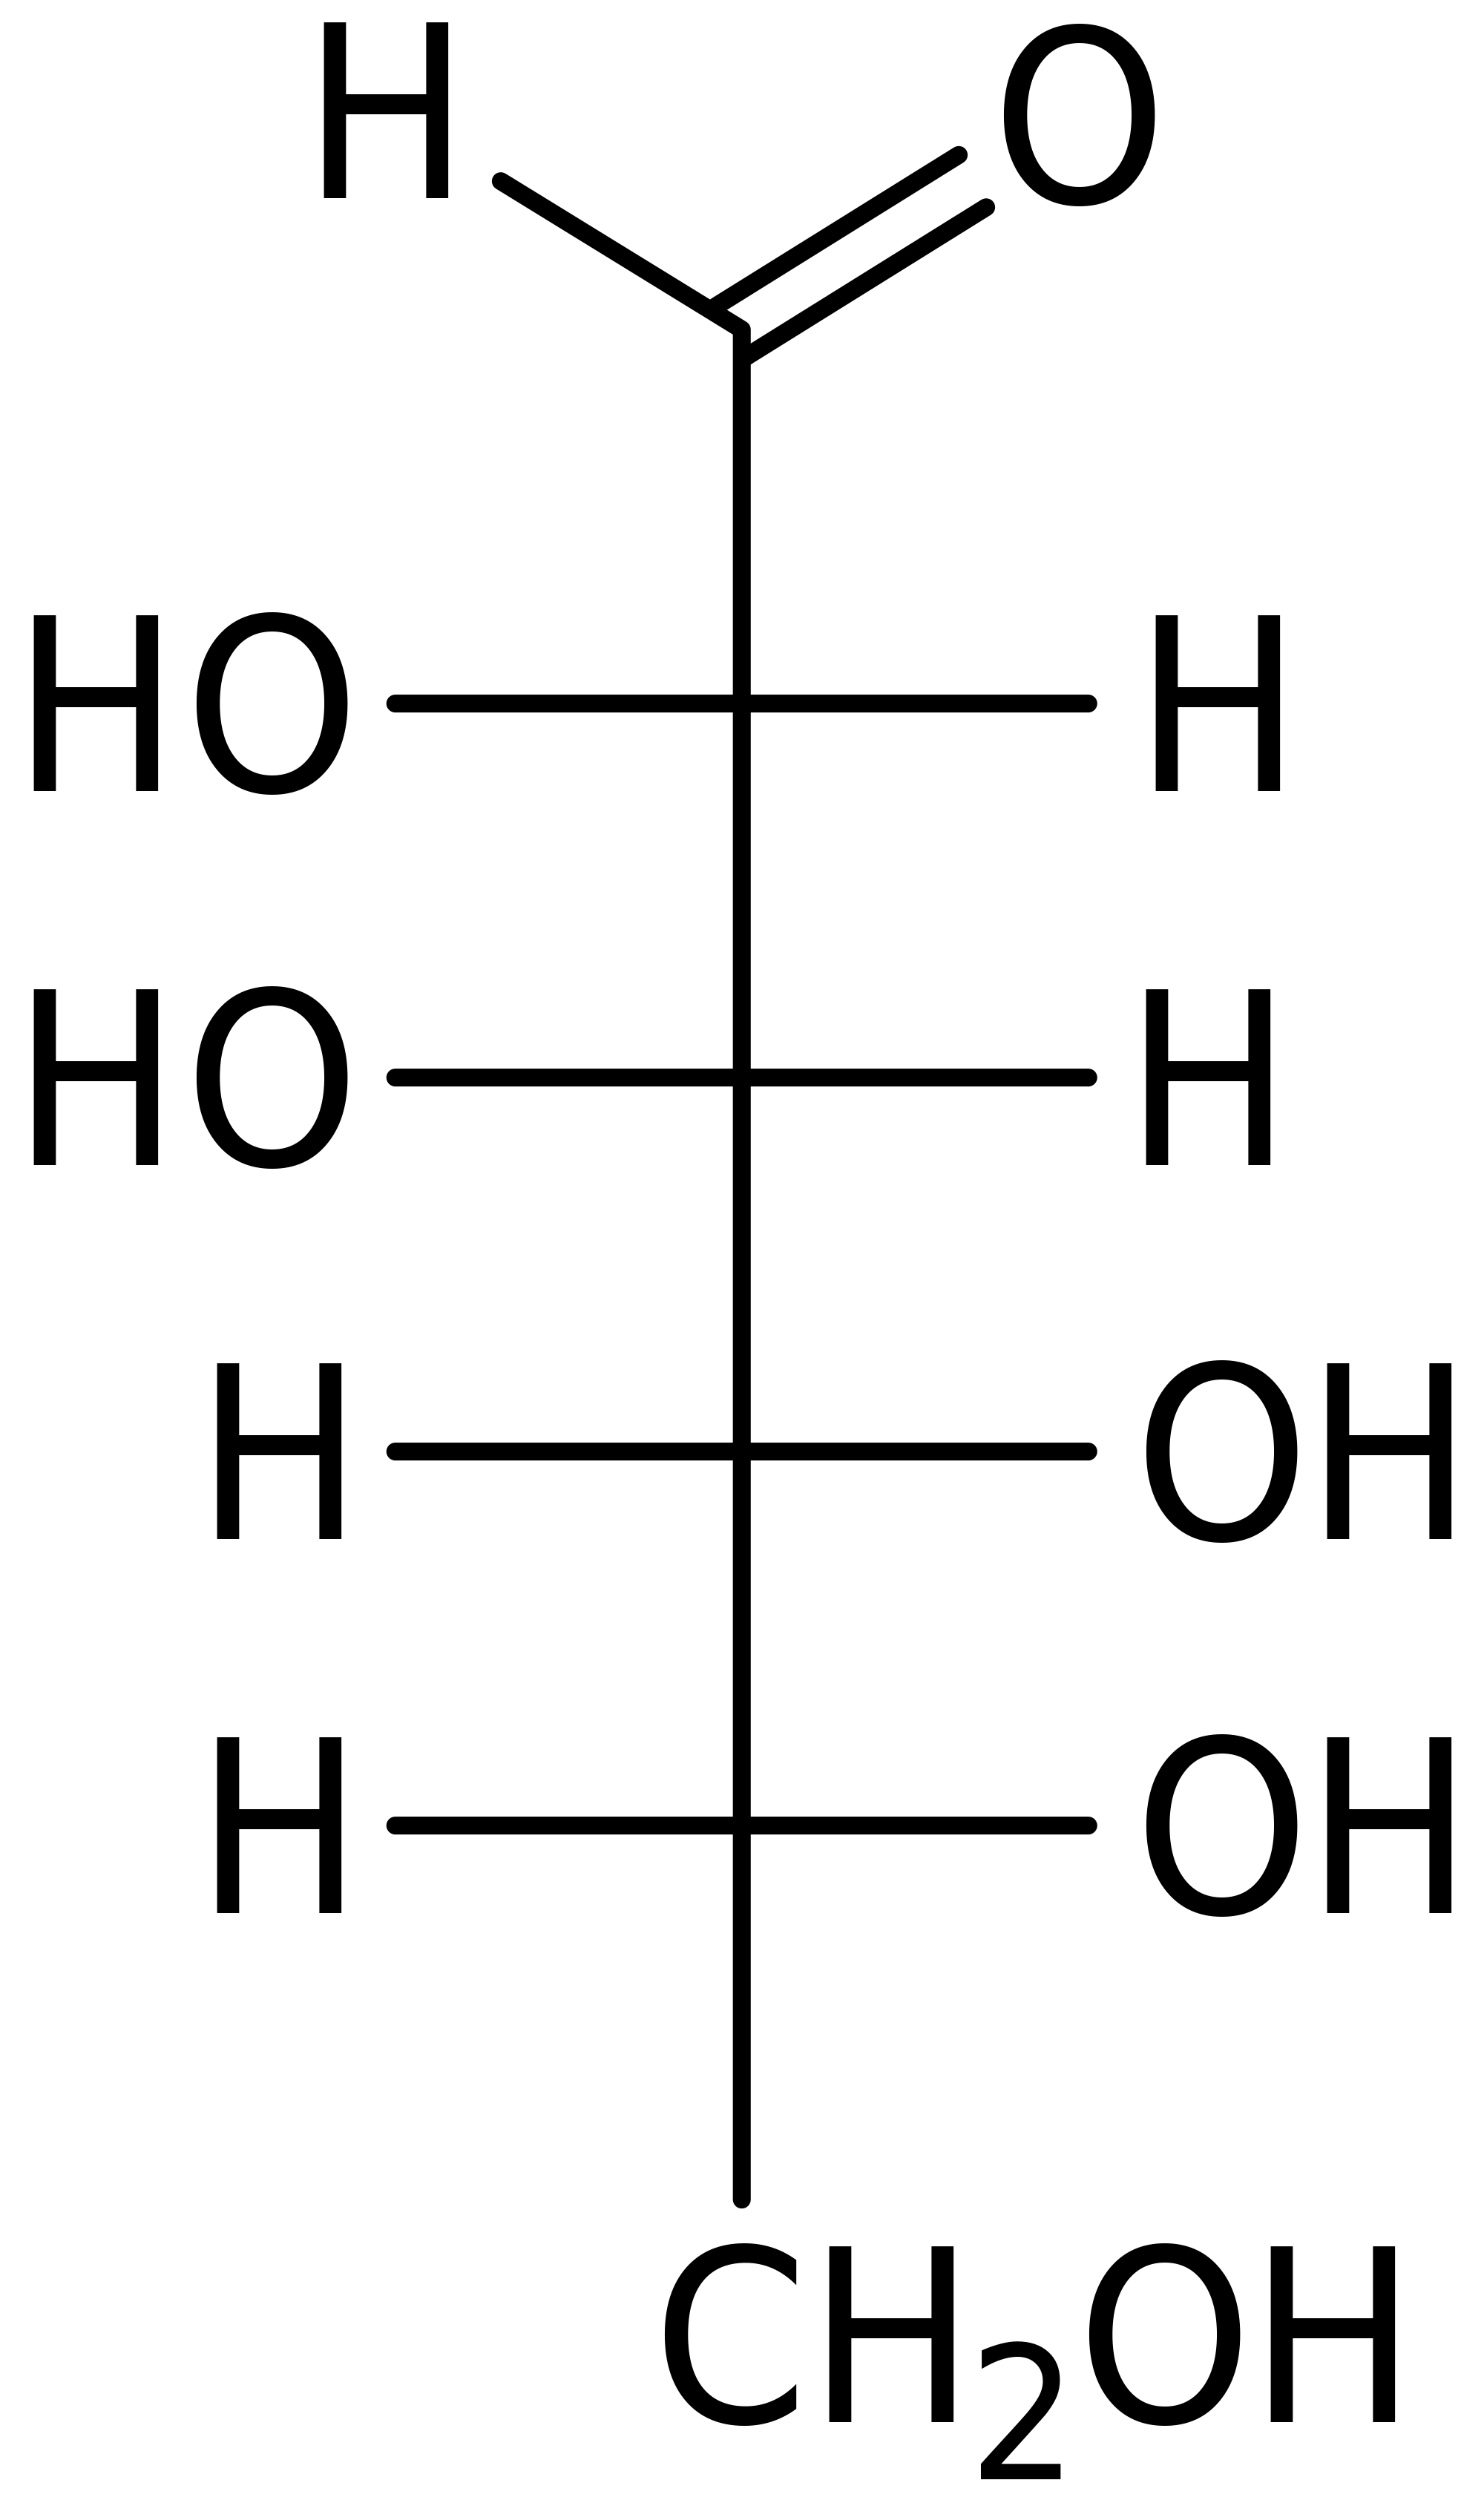
\includegraphics[width=0.2\textwidth]{images/mannose}\\
\\
\tab D-galaktóza:\\
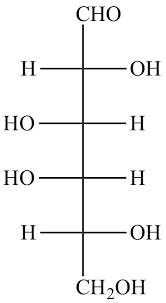
\includegraphics[width=0.2\textwidth]{images/galactose}\\
\tab D-ribóza:\\
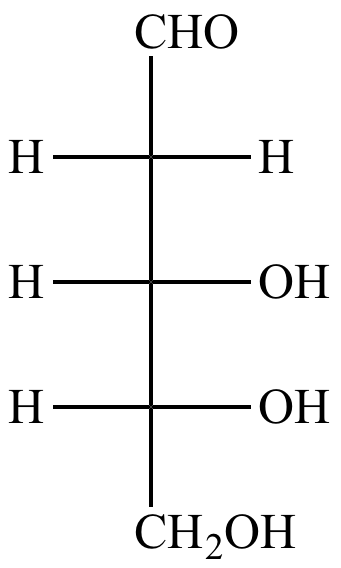
\includegraphics[width=0.2\textwidth]{images/ribose}\\
\subsection{Pojmy}
konfigurácia -- rozloženie, L alebo D
konformácia -- actuall 3D structure
enantiomér -- kompletne zrkadlové L a D. Nie iba ten spodný OH, ale všetky chirálne uhlíky\\
epiméry -- líšia sa iba v jednom chirálnom uhlíku OH-C-H $\rightarrow$ H-C-OH\\
diastereomér -- napr. D-aldohexóz je veľa, ale nie sú zrkadlové a neprekrývajú sa\\
poloacetál, poloketál -- keď alkoholový nukleofil reaguje s aldehydom/ketónom $\rightarrow$ acetál/ketál (ak je alkoholu dosť). Ale tu je len jeden OH, s ktorým to reaguje $\rightarrow$  poloacetál/poloketál $\rightarrow$ 
\tab vzniká pyranózový kruh (6 members)\\
\tab alebo furanóza (5 members a jeden trčí)\\
mutarotácia -- zmena rotácie sacharidu v pyranózovej/furanózovej forme medzi $\alpha$ a $\beta$ (opening, closing)\\
$\alpha$--trans, $\beta$--cis--anoméry -- stereoizoméry, kt sa líšia iba konfiguráciou na anomérnom uhlíku (ten, čo sa spája). $\alpha$-- OH dole, $\beta$ -- OH hore\\

\subsection{Vznik glykozidovej väzby}
hemiacetál $\rightarrow$ acetál\\
+ alkohol, -- voda\\
vznikne glykozid\\
na O na anomérnom uhlíku pribudne R z alkoholu (namiesto H)\\
väzba medzi O a anomérnym uhlíkom\\
Nie len alkohol -- napr. aj sacharidy dokopy\\
Opačne tiež -- hydrolýza\\
\subsection{Deriváty sacharidov}
\tab kyseliny\\
\tab \tab 1. uhlík $\rightarrow$ COOH (oxidácia slabými oxid čin)
Fehlingova reakcia -- oxidácia glukózy v alkalickom prostredí $\rightarrow$ 2, 3, 4, 6 uhlíkaté kyseliny
\tab \tab posledný uhlík $\rightarrow$ COOH (enzýmová oxidácia) $\rightarrow$ kys xxxx-urónová pre 6
		1. a 6. silnými oxidačnými čin $\rightarrow$ ald-árová
\tab alkoholy\\
\tab deoxysacharidy -- deoxyribóza\\
\tab estery sacharidov\\
\tab aminosacharidy -- glukozamín\\
\tab acetály\\
\tab ketály\\
\tab glykozidy\\
\subsection{Disacharidy}
\tab redukujúce\\
\tab neredukujúce disacharidy\\
\tab príklady -- laktóza\\
\tab sacharóza\\
\tab trehalóza\\
\subsection{Štruktúrne polysacharidy}
\tab celulóza\\
\tab chitín\\
\tab \tab väzby\\
\tab \tab štruktúra\\
\subsection{Zásobné polysacharidy}
\tab škrob\\
\tab glykogén
\tab \tab väzby\\
\tab \tab štruktúra\\
\subsection{Heteropolysacharidy}
\tab peptidoglykán\\
\tab hyaluronát\\
\tab proteoglykány (základná charakteristika)\\
\subsection{Sacharidy ako informačné molekuly}
\subsection{Lektíny}

%4
\section{Lipidy a biologické membrány DONE}

Status: DONE
Source: Prezentácia 3, 4

\subsection{Funkcie lipidov}
nerozpustnosť vo vode, iba v organických rozpúšťadlách\\
zásoba energie, membrány, kofaktory, prenášače e-, pigmenty, emulzifikátory, hormóny, signály vnútri bunky\\
\subsection{Štruktúra a vlastnosti mastných kyselín}

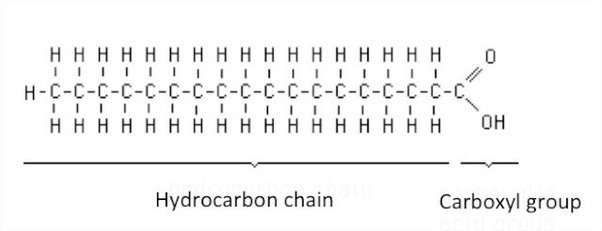
\includegraphics[width=0.5\textwidth]{images/fatty_acid}
\\
C4-C36 (38?), v lipidoch C14-C20 -- vyššie MK\\
párny počet C lebo pri vytváraní z A-CoA sa pridáva po 2\\
nerozvetvené\\
- (nasýtené vodíkom) aj = (nenasýtené vodíkom) väzby\\
CX, @Y -- X = počet uhlíkov, Y = ktorá väzba je dvojitá\\
\tab kyselina palmitová -- C16\\
\tab steárová -- C18\\
\tab olejová -- C18, @9\\
\tab linolová -- C18, @9, 12 \\
\tab linolénová -- C18, @9, 12, 15\\
čím viac = a čím kratší reťazec, tým nižšia teplota topenia\\
\tab pretože entropia ide dole s dĺžkou reťazca a hore s počtom dvojitých väzieb\\
\tab vyššia entropia $\rightarrow$ nižšia teplota topenia (menej pevné látky majú vyššiu entropiu)\\
\subsection{Triacylglyceroly}
zdroj energie, 3MK + glycerol $\rightarrow$ triacylglycerol + 3(H2O)\\
čím viac =, tým viac liquid\\
tuky -- prevažne živočíšne, viac nasýtených MK\\
oleje -- rastliny + ryby, viac nenasýtených MK\\
zdroj energie, lebo sú najredukovanejšia forma C v prírode, neviažu vodu, efektívne ukladanie\\
\subsection{glycerofosfolipidy}
polárna časť, nepolárna časť\\
glycerol + 2MK + PO4-alkohol/substituent\\

\includegraphics[width=0.5\textwidth, page=25]{materials/Biochemia/Prezentacie_Biochemia/03_Lipidy.pdf}
\includegraphics[width=0.5\textwidth, page=26]{materials/Biochemia/Prezentacie_Biochemia/03_Lipidy.pdf}
\\
fosfatidyletanolamín, fosfatidylcholín, fosfatidylserín, fosfatidylglycerol, fosfatidylinozitol, kardiolipín\\

\subsection{sfingolipidy}

\includegraphics[width=0.5\textwidth, page=30]{materials/Biochemia/Prezentacie_Biochemia/03_Lipidy.pdf}
\includegraphics[width=0.5\textwidth, page=31]{materials/Biochemia/Prezentacie_Biochemia/03_Lipidy.pdf}
\\
sfingomyelíny, cerebrozidy, ceramidy, gangliozidy\\

\subsection{vosky}
estery MK + OH s dlhými reťazcami\\
zdroj energie, ochranná funkcia\\
včelí vosk -- kys palmitová + triacontatol\\

\subsection{cholesterol}
štruktúra a funkcia\\
\tab polárna hlavička, steroidné jadro, alkylový bočný reťazec\\
\tab prekurzor na kortizol (metabolizmus, imunita), estradiol (pohl. Hormóny)\\

\subsection{Amfipatický charakter niektorých lipidov}
časť hydrofilná, časť hydrofóbna\\
fosfolipidy\\
\subsection{agregované formy lipidov}
micely -- guličky\\
dvojvrstvy\\
lipozómy -- dvojvrstvová gulička\\
\subsection{Princíp samovoľného vzniku lipidových agregátov}
hydrofóbne dnu, hydrofilné von\\
\subsection{Biomembrány}
Kompartmentalizácia, styk s okolím, ohraničenie bunky/organely, priestor na metabolické deje\\
membránové proteíny\\
\tab integrálne -- ide cez membránu\\
\tab periférne -- na povrchu\\
model tekutej mozaiky\\
\tab zložené z veľa rôznych komponentov -- fosfolipidy, glykolipidy (rozoznávanie buniek, krvné skupiny), proteíny, cholesterol\\
\subsection{Úloha cholesterolu pri ovplyvňovaní fluidity membrán}
pri nízkych teplotách zabráni fosfolipidom sa pritisnúť k sebe $\rightarrow$ zvyšuje fluiditu\\
pri vysokých teplotách im bráni sa hýbať rýchlo $\rightarrow$ znižuje fluiditu\\
\subsection{Transport cez membrány}
flipáza -- otáča fosfolipidy\\
pasívny -- v smere koncentračného spádu, energeticky výhodný\\
\tab difúzia
aktívny -- treba energiu\\
\tab primárny -- energia z hydrolýzy ATP\\
\tab sekundárny -- poháňaný koncentračným spádom\\
$Na^+/K^+$ pumpa.\\
\tab $Na^+$ von, $K^+$ dnu
\\
%5
\section{Enzýmy DONE}

Status: DONE
Source: Prezentácia 4, 5

\subsection{Význam enzýmovej katalýzy}
Regulácia rýchlosti reakcií\\
proteíny, špecifikácia\\
\subsection{Pojmy}
holoenzým -- kompletný aktívny enzým s naviazaným kofaktorom\\
apoenzým -- proteínová zložka holoenzýmu (nie nutne aktívny)\\
kofaktor -- ión kovu alebo koenzým, priamo pomáha s katalýzou\\
koenzým -- organická molekula, carrier (napr NADH je \el carrier $\rightarrow$ NAD+ + H, CoA je acyl carrier)\\
prostetická skupina -- kofaktor pevne (kovalentne) viazaný v enzýme\\
apoenzým + kofaktor $\rightarrow$ holoenzým
\subsection{Klasifikácia enzýmov}
oxido-reduktázy -- prenos \el, protónov
transferázy -- prenos skupín, aminoacids to to peptide chain
hydrolázy -- hydrolytické reakcie, A + H2O $\rightarrow$ B + C
Lyázy -- odštiepenie skupín, tvorba dvojitých väzieb, A $\rightarrow$ B + C
izomerázy -- vznik izomérov
ligázy -- tvorba C-C, C-S, C-N, C-O a fosfoesterových väzieb, pri tvorbe ATP, A + B $\rightarrow$ AB, spájanie strands of DNA
\subsection{Aktívne miesto, špecificita enzýmov}
substrát sa viaže do aktívneho miesta, tvorí komplex enzým-substrát\\
aktívne miesto obsahuje katalytické centrum a väzobné centrum\\
zníženie aktivačnej energie\\
väzba substrátu -- slabé interakcie\\
štruktúrna komplementarita $\rightarrow$ rozpoznávanie\\

Jednotka enzýmovej aktivity -- katal\\
\tab množstvo enzýmu, kt katalyzuje 1 mol substrátu za 1 sekundu
\tab špecifická aktivita = katal/kg bielkoviny
\subsection{Mechanizmus účinku enzýmov}
teória komplementarity -- substrát do enzýmu “zapadne”, špecificky, nevie do iného\\
teória indukovaného prispôsobenia -- substrát nie úplne zapadne, enzým sa mierne prispôsobí\\
\subsection{Termodynamické hľadisko priebehu enzymaticky katalyzovaných reakcií}
aktivačná energia -- energia potrebná na prebehnutie reakcie\\
prechodný stav -- niekde medzi produktom a substrátom, reakcia prebieha\\
\subsection{Kinetické hľadisko priebehu enzymaticky katalyzovaných reakcií}
faktory ovplyvňujúce rýchlosť enzýmovej reakcie\\
\tab množstvo enzýmu, koncentrácia substrátov, fyz-chem vlastnosti prostredia (t, pH), efektory (aktivátory, inhibítory)\\
Michaelis -- Mentenovej rovnica\\
\tab $V_0 = {{V_{max} [S]} \over {K_m + [S]}}$\\
\tab $[S]$ -- koncentrácia substrátu\\
\tab parametre $K_m$ a $V_{max}$\\
\tab \tab $K_m$ -- Michaelis-Mentenovej konštanta -- koncentrácia substrátu, keď rýchlosť $V_0 = {V_{max}\over 2}$\\
\tab \tab $V_{max}$ -- maximálna rýchlosť reakcie\\
\tab \tab $K_m$ nižšia $\rightarrow$ afinita enzýmu ku substrátu vyššia\\
\subsection{inhibícia enzýmov}
ireverzibilná - inhibítor sa viaže pevne, až kovalentne\\
reverzibilná - nekovalentné, slabšie interakcie\\
\tab kompetetívna -- nepustí substrát dnu\\
\tab nekompetetívna -- pustí aj substrát\\
\subsection{Regulácia enzýmov}
alosterickou modifikáciou -- z neaktívnej strany sa naviaže inhibítor/aktivátor, kt ovplyvní aktívnu stranu\\
kovalentnou modifikáciou -- formovanie/ničenie kovalentných väzieb, napr. metylácia, acylácia, fosforylácia\\
regulačnými proteínmi -- tripsinogén je aktivovaný na tripsín, nevratne\\
proteolytickým štiepením (zymogény) -- odíde kus enzýmu a odhalí sa aktívne miesto, napr. v golgiho aparáte\\
\\
%6
\section{Základy metabolizmu DONE}

Status: DONE
Source: Prezentácia 5

\subsection{Zdroj a premeny energie v biosfére}
I zákon termodynamický -- konštantné množstvo energie, mení sa len forma\\
II zákon termodynamický -- entropia spontánne vzrastá\\
Chemická energia -- entalpia -- energia chemickej väzby\\
voľná (Gibbsova) energia -- časť energie v štruktúre molekúl, ktorá sa môže premeniť na prácu\\
entropia -- miera chaose\\
Exergonické reakcie -- $\Delta G < 0$ -- energia sa uvoľní\\
Endergonické reakcie -- $\Delta G> 0$ -- energia sa spotrebuje\\
Podmienka samovoľnosti priebehu chemických dejov -- $\Delta G < 0$\\
\subsection{Význam prenášačov energie}
dodávajú energiu z exergponických reakcií do endergonických\\
sú schopné energiu zachytiť a uložiť, uvoľniť a odovzdať\\
napr. ATP\\
\subsection{vznik ATP}
substrátová fosforylácia\\
oxidačná fosforylácia\\
fotofosforylácia\\
\subsection{premeny ATP}
Katabolické a anabolické metabolické dráhy, ich význam\\
\tab živiny s vysokým obsahom energie $\rightarrow$ katabolizmus $\rightarrow$ koncové produkty s málo energie\\
\tab prekurzorové molekuly $\rightarrow$ anabolizmus $\rightarrow$ makromolekuly\\
Energetické vzťahy medzi katabolickými a anabolickými dráhami\\

\subsection{Oxidácia biomolekúl}
oxidácia -- strata \el, berú ich biomolekulám
\\
%7
\section{Metabolizmus sacharidov +-DONE}

Status: More or less
Source: Prezentácia 6

\subsection{Glukóza ako zdroj metabolickej energie}
štruktúra, zásoba, oxidácia glykolýzou $\rightarrow$ pyruvát, pentózovou dráhou $\rightarrow$ ribóza-5-fosfát\\
\subsection{Glykolýza}
\tab význam -- glukóza $\rightarrow$ pyruvát (ATP, NADH)\\
\tab lokalizácia -- cytoplazma
\tab 2 fázy glykolýzy\\
\tab \tab prípravná (5 reakcií), produkčná (5 reakcií)
\tab jednotlivé reakcie\\
\tab \tab fosforylácia glukózy $\rightarrow$ glyceraldehyd-3-fosfát\\
\tab \tab glyceraldehyd-3-fosfát $\rightarrow$ pyruvát, ATP, NADH\\
\tab medziprodukty a enzýmy glykolýzy\\
Spotreba a vznik ATP počas glykolýzy\\
\includegraphics[width=0.5\textwidth, page=6]{materials/Biochemia/Prezentacie_Biochemia/06_Glyko_Gluko_Pento.pdf}
\includegraphics[width=0.5\textwidth, page=7]{materials/Biochemia/Prezentacie_Biochemia/06_Glyko_Gluko_Pento.pdf}
\\
substrátová fosforylácia\\
\subsection{Osud pyruvátu a regenerácia NAD+}
anaeróbne -- mliečne kvasenie\\
alkoholové kvasenie\\
aeróbne -- v dýchacom reťazci\\
\subsection{Glukoneogenéza}
význam -- potreba tela vyrobiť si vlastnú glukózu\\
substráty\\
\tab pyruvát, laktát, mnohé AK, glycerol, veci z krebsovho cyklu\\
\tab nie MK, lebo idú na Acetyl-CoA oxidovaný v Krebsovom cykle\\
tri unikátne glukoneogenetické kroky (4 enzýmy)\\
lokalizácia\\
\tab králik -- mitochondrie, potkan -- cytoplazma, človek -- obe\\
\\
\\
\subsection{Coriho cyklus}
prenos laktátu zo svalu do pečene\\
vznik glukózy z laktátu procesom glukoneogenézy\\
Pentózová dráha: 
\tab význam -- NADPH pre biosyntézy, produkcia ribóza-5-P\\
\tab východisková zlúčenina -- Glc-6-P\\
\tab vznik NADPH, ribóza--5--fosfátu\\
\tab reakcie katalyzované dehydrogenázami, izomerázou, epimerázou, transaldolázami, transketolázami.\\
\\
%8
\section{Citrátový cyklus}
Glyoxylátový cyklus\\
Vznik acetyl--koenzýmu A z kyseliny pyrohroznovej.\\
Citrátový cyklus -- zdroj energie a biosyntetických prekurzorov\\
\tab bunková lokalizácia cyklu\\
Reakcie\\
citrátového cyklu\\
\tab jednotlivé medziprodukty a enzýmy\\
Vznik redukovaných koenzýmov\\
Tvorba\\
GTP -- substrátová fosforylácia\\
Amfibolický charakter citrátového cyklu\\
\tab anaplerotické reakcie\\
(pyruvátkarboxyláza)\\
Glyoxylátový cyklus -- význam pre rastliny a baktérie\\
\tab lokalizácia (spolupráca\\
glyoxyzómov a mitochondrií)\\
\tab enzýmy.\\
\\
%9
\section{Oxidačná fosforylácia}
Štruktúra a funkcia mitochondrií\\
Zloženie a funkcia dýchacieho reťazca,\\
prenášače elektrónov -- cytochrómy\\
\tab bielkoviny s nehemovo viazaným železom\\
\tab ubichinón,\\
flavoproteíny\\
Zdroj elektrónov vstupujúcich do dýchacieho reťazca\\
Prenos elektrónov v dýchacom\\
reťazci (komplexy I\\
\tab II\\
\tab III\\
\tab IV\\
\tab cyt c\\
\tab ubichinón)\\
Vznik protónového gradientu\\
Využitie protónového\\
gradientu na syntézu ATP\\
\tab enzým ATP--syntáza\\
Chemiosmotická teória\\
Ďalšie možnosti využitia\\
protónového gradientu -- termogenéza\\
\tab pohyb baktérií\\
\tab transport metabolitov.\\
\\
%10
\section{Fotosyntéza}
\subsection{Fotofosforylácia ako súčasť fotosyntézy}
\subsection{Štruktúra a funkcia chloroplastov}
\subsection{Pigmenty a ich úloha v procese fotosyntézy}
\subsection{Fotochemické reakčné centrum a deje, ktoré v ňom prebiehajú}
\subsection{Prenos elektrónov fotosystémami I a II}
\subsection{Necyklická a cyklická fotofosforylácia}
\subsection{Fotolýza vody}
\subsection{Vznik NADPH a ATP}
\subsection{Spoločné a rozdielne znaky fotofosforylácie a oxidačnej fosforylácie}
\subsection{Syntézasacharidov počas fotosyntézy}
\subsection{Tri štádiá asimilácie CO2}
\subsection{Základné reakcie a funkcia Calvinovhocyklu}
%11
\section{Metabolizmus lipidov +-DONE}

Status: Better than nothing
Source: Prezentácia 10

\subsection{Mastné kyseliny ako zdroj metabolickej energie}
najredukovanejšia forma uhlíka\\
nerozpustnosť vo vode\\
chemicky inertné\\
\subsection{Trávenie tukov}
význam žlčových kyselín\\
\tab emulzifikácia tukov z potravy, tvorba miciel
enzýmy lipáz\\
\tab degradácia triglycerolov\\
chylomikróny\\
\tab prenos premenených tukov ku tkanivám\\
\subsection{Osud mastných kyselín vo svaloch a v tukovom tkanive}
Oxidácia $\rightarrow$ zdroj energia alebo reesterifikácia $\rightarrow$ zásoby energie
Uvoľnenie mastných kyselín z tukového tkaniva a ich prenos do tkanív\\
\tab chylomikróny
funkcia sérumalbumínu\\
\tab proteín, prenáša MK
\subsection{$\beta$--oxidácia mastných kyselín}
lokalizácia v bunke\\
prenos mastných kyselín do mitochondrií\\
\tab (funkcia karnitínu)\\
\subsection{Reakcie $\beta$--oxidácie}
dehydrogenácia\\
hydratácia\\
dehydrogenácia\\
štiepenie\\
vznik acetyl--kaoenzýmu A\\
Osud acetyl--koenzýmu A\\
\tab vstup do citrátového cyklu\\
vznik ketolátok, ich význam\\
\tab zdroj energie pre niektoré tkanivá, napr. mozog, srdce, obličky\\
\tab počas hladovania\\
\tab MK sa oxidáciou v pečeni premieňajú na acetón, etc.\\
\subsection{Biosyntéza mastných kyselín}
porovnanie s $\beta$--oxidáciou\\

\includegraphics[width=0.5\textwidth, page=24]{materials/Biochemia/Prezentacie_Biochemia/10_Met_MK.pdf}

východiskové zlúčeniny\\
reakcie kondenzácia\\
redukcia\\
dehydratácia\\
\subsection{Zdroje NADPH}
malát $\rightarrow$ pyruvát\\
pentózová dráha\\
\subsection{Transport triacylglycerolov a cholesterolu u ľudí}
zabezpečujú lipoproteíny a chylomikróny\\
\\

%12
\section{Degradácia aminokyselín DONE}

Status: hopefully DONE
Source: Prezentácia 11

Močovinový cyklus\\
Počas bežnej degradácie a syntézy v bunkách (AK sa neukladajú do zásoby)\\
Ak je priveľa AK v potrave\\
\subsection{Aminokyseliny ako zdroj metabolickej energie}
Keď nie sú k dispozícii sacharidy ako zdroj\\
\subsection{Odbúranie aminokyselín}
Odstránenie aminoskupiny transamináciou a deamináciou\\
enzýmy transaminázy, glutamátdehydrogenáza\\
\subsection{Význam glutamínu pri odbúraní AK}
Glutamát + amoniak $\rightarrow$ glutamín $\rightarrow$ mitochondrie pečene/obličiek $\rightarrow$ amoniak sa uvoľní $\rightarrow$ močovinový cyklus\\
enzýmy glutamínsyntetáza -- naviazanie amoniaku\\
glutamináza -- uvoľnenie amoniaku\\
\subsection{Formy vylučovania aminoskupiny u rôznych stavovcov}
amoniak -- vodné stavovce\\
močovina -- suchozemské stavovce\\
kys. močová -- vtáky, plazy\\
\subsection{Močovinový cyklus -- orgánová a bunková lokalizácia, význam}
V cytoplazme pri mitochondriách\\
arginínosukcinát spoločný s citrátovým cyklom\\
\subsection{Osud uhlíkovej kostry aminokyselín}
premena na glukózu/ketolátky, podľa typu AK\\
glukogénne AK $\rightarrow$ pyruvát, etc. (nejakú látku citrátového cyklu)
ketogénne AK $\rightarrow$ acetyl-CoA, etc.
